% The morphism of short exact sequences relating the ray class data
% for the modulus 15∞ to the modulus 5∞.
% Source: book/tex/alg-NT/artin.tex (§ Application, example) — tikzcd.
\documentclass[border=2mm]{standalone}
\usepackage{tikz}
\usetikzlibrary{arrows.meta}
\usepackage{amssymb}
\usepackage{amsmath}
\begin{document}
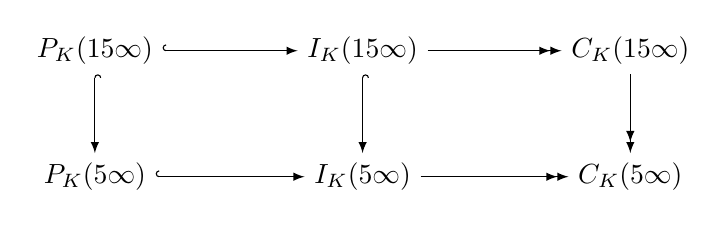
\begin{tikzpicture}[>=latex]
  \node (P1) at (0,1.6) {$P_K(15 \infty)$};
  \node (I1) at (3.4,1.6) {$I_K(15 \infty)$};
  \node (C1) at (6.8,1.6) {$C_K(15 \infty)$};
  \node (P2) at (0,0) {$P_K(5 \infty)$};
  \node (I2) at (3.4,0) {$I_K(5 \infty)$};
  \node (C2) at (6.8,0) {$C_K(5 \infty)$};
  \draw[{Hooks[right]}->] (P1) -- (I1);
  \draw[->>] (I1) -- (C1);
  \draw[{Hooks[right]}->] (P2) -- (I2);
  \draw[->>] (I2) -- (C2);
  \draw[{Hooks[right]}->] (P1) -- (P2);
  \draw[{Hooks[right]}->] (I1) -- (I2);
  \draw[->>] (C1) -- (C2);
\end{tikzpicture}
\end{document}
